% This must be in the first 5 lines to tell arXiv to use pdfLaTeX, which is strongly recommended.
\pdfoutput=1
% In particular, the hyperref package requires pdfLaTeX in order to break URLs across lines.


\documentclass[11pt]{article}


% Change "review" to "final" to generate the final (sometimes called camera-ready) version.
% Change to "preprint" to generate a non-anonymous version with page numbers.
\usepackage{acl}

% Standard package includes
\usepackage{times}
\usepackage{latexsym}
\usepackage{rotating}
\usepackage{natbib}
\usepackage{varioref}  
\usepackage{graphicx}


% For proper rendering and hyphenation of words containing Latin characters (including in bib files)
\usepackage[T1]{fontenc}
% For Vietnamese characters
% \usepackage[T5]{fontenc}
% See https://www.latex-project.org/help/documentation/encguide.pdf for other character sets

% This assumes your files are encoded as UTF8
\usepackage[utf8]{inputenc}

% This is not strictly necessary, and may be commented out,
% but it will improve the layout of the manuscript,
% and will typically save some space.
\usepackage{microtype}

% This is also not strictly necessary, and may be commented out.
% However, it will improve the aesthetics of text in
% the typewriter font.
\usepackage{inconsolata}

%Including images in your LaTeX document requires adding
%additional package(s)
\usepackage{graphicx}
\usepackage{setspace}
\usepackage{graphicx}
\usepackage{listings}
\usepackage{xcolor}
\usepackage{subcaption}
\usepackage{import}

\usepackage{cleveref}

% Custom command for appendix figures
\newcommand{\appfigure}[1]{Figure~\ref{#1}}


% Add this line to define \textrussian command
\newcommand{\textrussian}[1]{\foreignlanguage{russian}{#1}}

\lstset{
    language=Python,
    breaklines=true,
    basicstyle=\small\ttfamily,  % Reduced font size
    keywordstyle=\color{blue}\bfseries,  % Bold blue keywords
    stringstyle=\color{green!50!black},  % Dark green strings
    commentstyle=\color{gray}\itshape,  % Italic gray comments
    numbers=left,  % Add line numbers on the left
    linewidth=0.5\textwidth,  % Increased width to 95% of text width
    showspaces=false,
    showstringspaces=false,  % Don't show spaces in strings
    captionpos=b,  % Place caption at the bottom
    tabsize=4,  % Set tab size to 4 spaces
    keepspaces=true,  % Keep spaces in code
    xleftmargin=\parindent,  % Align with paragraph indentation
}
\usepackage{graphicx}
\graphicspath{{../plots/}}



\begin{document}

\nolinenumbers  % Add this line to ensure line numbers are turned off


\title{NLP Course Report}
\author{Group members: pvr448}

\maketitle

\section{Attribution}
this report was in in its entirety written by, pvr448.

\section{Week 36}
\label{week36}
% (a) Explore the dataset from https://huggingface.co/datasets/coastalcph/tydi_xor_rc. 
% Familiarize yourself with the dataset card, download the dataset and explore its columns. 
% Summarize basic data statistics for training and validation data in each of the languages 
% Fi, Ja and Ru.
\begin{enumerate}
    \item[(a)] 

    Basic statistics:
    \begin{itemize}
        \item The data is relatively evenly distributed across the three languages.
        \item There is a notable imbalance between answerable and unanswerable questions, with a ratio of approximately 10:1. This imbalance suggests that accuracy alone would be an insufficient metric for evaluation.
        \item Training set size: 15,326 samples
        \item Validation set size: 3,028 samples
    \end{itemize}

    \begin{figure}[ht]
        \centering
        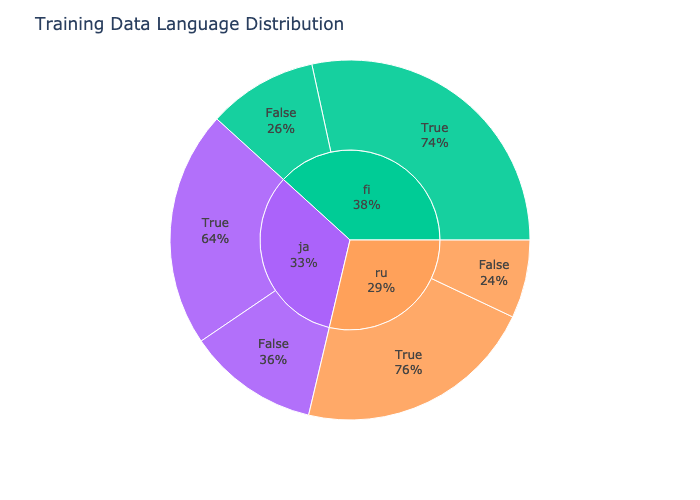
\includegraphics[width=0.3\textwidth]{week1_a_dataset.png}
        \caption{Distribution of labels in the dataset}
        \label{fig:label_distribution}
    \end{figure}

    \begin{figure}[ht]
        \centering
        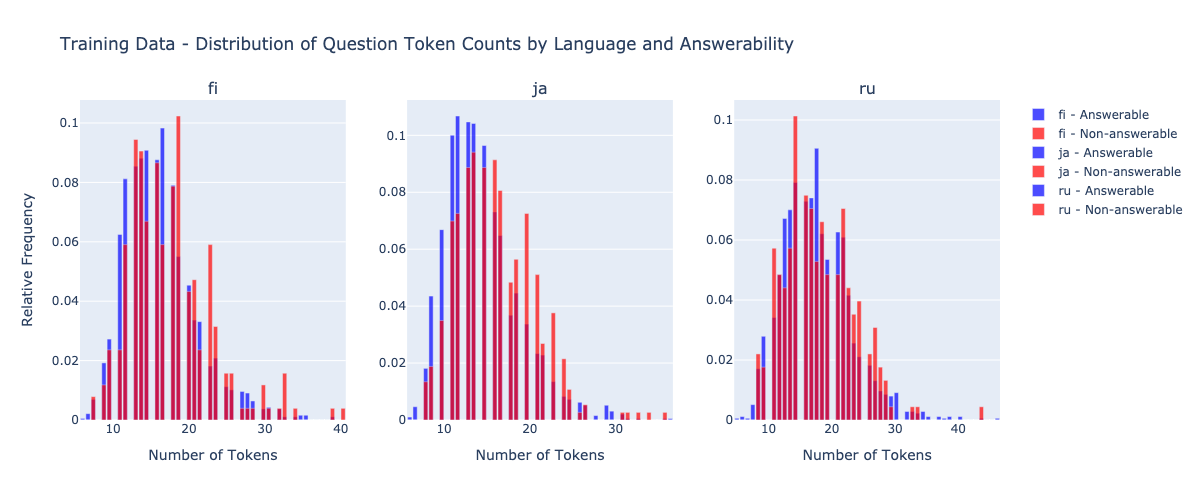
\includegraphics[width=0.5\textwidth]{week1_a_lang_token_distribution_normalized.png}
        \caption{Normalized histogram of token counts (using Llama-3 tokenizer) for answerable and unanswerable questions in the dataset}
        \label{fig:language_distribution}
    \end{figure}

    % (b) For each of the languages Finnish, Japanese and Russian, report the 5 most common 
    % words in the questions from the training set. What kind of words are they?
    \item[(b)] 

    To obtain a meaningful representation of the most informative words, we employed the following methodology:
    \begin{itemize}
        \item Filtered out stopwords using spaCy's language-specific stopword lists
        \item Removed common symbols and tokens not included in the stopword lists
        \item For Finnish and Russian, which use space-delimited words, we extracted distinct words by splitting on spaces
        \item For Japanese, which does not use spaces to delimit words, we employed a language-specific tokenizer
    \end{itemize}

    The results are presented in Figure~\ref{fig:top_5_tokens_all}:

    \begin{figure}[t]
        \centering
        \begin{subfigure}[b]{0.1\textwidth}
            \centering
            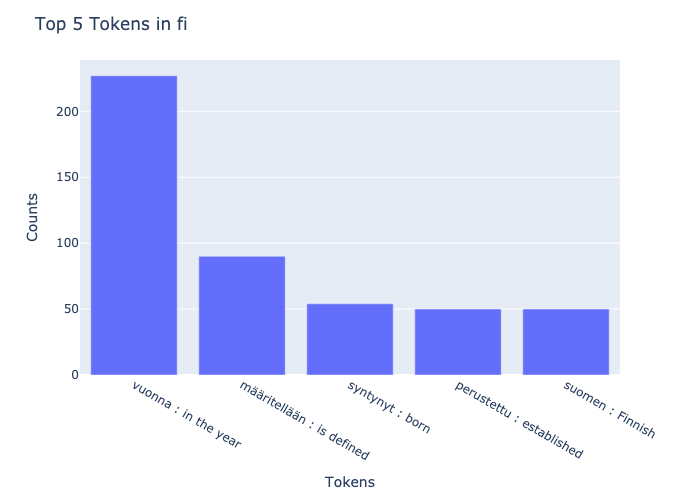
\includegraphics[width=\textwidth]{week1_b_top_5_tokens_fi.png}
            \caption{Finnish}
            \label{fig:top_5_tokens_fi}
        \end{subfigure}
        \hfill
        \begin{subfigure}[b]{0.1\textwidth}
            \centering
            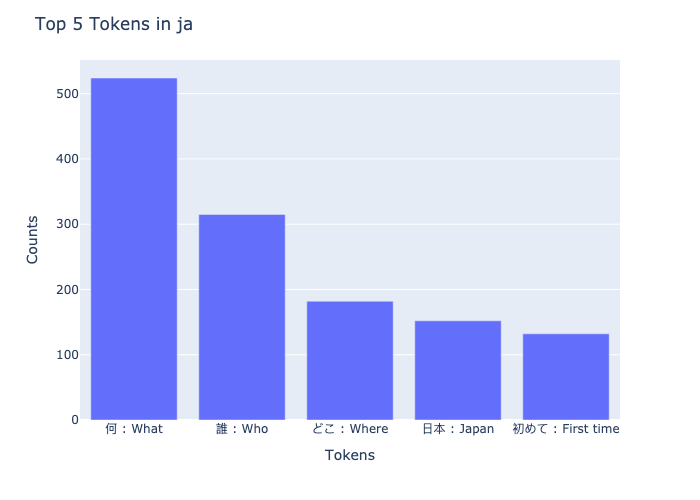
\includegraphics[width=\textwidth]{week1_b_top_5_tokens_ja.png}
            \caption{Japanese}
            \label{fig:top_5_tokens_ja}
        \end{subfigure}
        \hfill
        \begin{subfigure}[b]{0.1\textwidth}
            \centering
            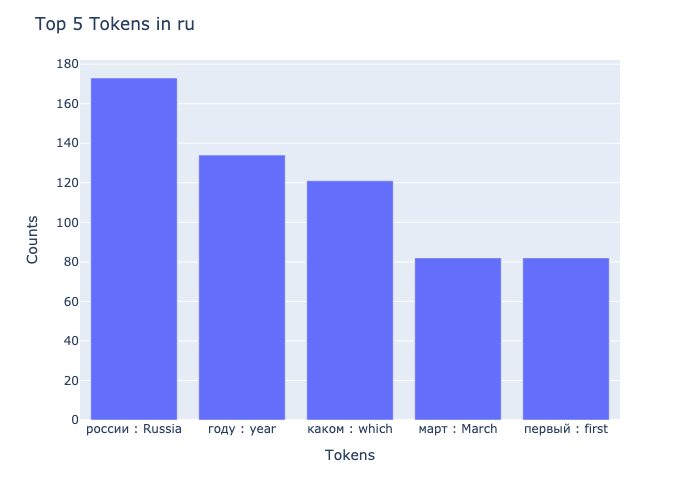
\includegraphics[width=\textwidth]{week1_b_top_5_tokens_ru.png}
            \caption{Russian}
            \label{fig:top_5_tokens_ru}
        \end{subfigure}
        \caption{Top 5 tokens in Finnish, Japanese, and Russian}
        \label{fig:top_5_tokens_all}
    \end{figure}

    Across all three languages, we observe several commonalities:
    \begin{itemize}
        \item Words related to time, such as 'year' or 'year of', consistently appear in the top 5
        \item The names of the respective capital cities are prominent in all three languages
        \item Other common words include 'first' and various prepositions
    \end{itemize}

    In general, the most frequent words tend to be those that help describe facts or serve as prepositions, which is consistent with the question-answering nature of the dataset.

    % (c) Implement a rule-based classifier that predicts whether a question is answerable 
    % or impossible, only using the document (context) and question. You may use machine 
    % translation as a component. Use the answerable field to evaluate it on the validation set. 
    % What is the performance of your classifier for each of the languages Finnish, Japanese and Russian?
    \item[(c)] 
    
    Based on the hypothesis that longer questions might be more challenging to answer, we implemented a simple rule-based classifier. We plotted the question word length against the answerability for each language (see Figures~\ref{fig:scatter_week1_c_fi}, \ref{fig:scatter_week1_c_ja}, and \ref{fig:scatter_week1_c_ru}). A slight correlation between question length and answerability was observed.

    Our classifier predicts a question as unanswerable if its length exceeds a language-specific threshold determined from these scatter plots. The performance of this classifier on the validation set is presented in Table~\ref{tab:classifier_performance}.

    \begin{table}[ht]
        \centering
        \resizebox{0.9\columnwidth}{!}{
        \begin{tabular}{|l|c|c|c|c|}
            \hline
            Language & Balanced Accuracy & F1 Score & Precision & Recall \\
            \hline
            All & 0.5284 & 0.7834 & 0.7032 & 0.8843 \\
            Fi & 0.5133 & 0.8107 & 0.7256 & 0.9184 \\
            Ja & 0.5375 & 0.6908 & 0.6542 & 0.7317 \\
            Ru & 0.4965 & 0.8319 & 0.7157 & 0.9930 \\
            \hline
        \end{tabular}
        }
        \caption{Performance metrics of the rule-based classifier on the validation set}
        \label{tab:classifier_performance}
    \end{table}

    The performance of this rule-based classifier is suboptimal, which can be attributed to several factors:
    \begin{itemize}
        \item While question length may correlate with answerability to some extent, it is a noisy signal and an imperfect proxy for question complexity
        \item The effectiveness of the classifier is heavily dependent on the tokenization method used, which may introduce inconsistencies across languages
        \item The performance is only marginally better than random guessing based on the prior distribution of answerable questions in the training data
    \end{itemize}

    These limitations highlight the need for more sophisticated approaches to accurately classify question answerability in this multilingual dataset.

\end{enumerate}

\section{Week 37 (9--15 September)}
\label{sec:week37}
% Let k be the number of members in your group (k ∈ {1, 2, 3}). Implement k different 
% language models for the questions in the three languages Finnish, Japanese and Russian, 
% as well as for the document contexts in English (total k × 4 language models), using the 
% training data. Evaluate each of them on the validation data, report their performance 
% and discuss the results.

We implemented four distinct N-Gram models, one for each language under consideration. 
The implementation leverages the Natural Language Toolkit (NLTK) for core language processing tasks, incorporating the Lidstone smoothing method to ensure the model can effectively handle unseen word combinations without yielding extreme perplexities.
For training, we employed the tokenization techniques described in Section \ref{week36}. We trained on the entire training set, utilizing a model with order=2.

\begin{table}[ht]
    \centering
    \resizebox{0.9\columnwidth}{!}{%
    \begin{tabular}{|l|r|r|}
        \hline
        Language & Training Tokens/Words & Perplexity \\
        \hline
        Japanese & 24,533 & 432.04 \\
        Russian & 16,526 & 133.03 \\
        Finnish & 13,013 & 88.50 \\
        Context (English) & 751,154 & 593.63 \\
        \hline
    \end{tabular}
    }
    \caption{Language Model Performance}
    \label{tab:language_model_performance}
\end{table}

Interestingly, we observed that as the number of tokens in the training data increases, the performance of the model deteriorates. 
This phenomenon is consistent across all four models and persists when training based on the last 3, 2, or 1 tokens. 
We found that the N-gram model performs poorly, with perplexity increasing as the number of training tokens grows. Moreover, every model except the one trained on the context performs optimally when order=1, indicating that the model relies solely on the previous word to predict the next word.
We refer to the appendix for a detailed scaling analysis, as shown in Figures~\ref{fig:week2_scaling_ja}, \ref{fig:week2_scaling_fi}, \ref{fig:week2_scaling_ru}, and \ref{fig:week2_scaling_context}.  

\section{Week 38 (16--22 September)}
\label{sec:week38}
% Let k be the number of members in your group. For each of the three languages Finnish, 
% Japanese and Russian separately, using the training data, train k different classifiers 
% that receive the document (context) and question as input and predict whether the question 
% is answerable or impossible given the context. Evaluate the classifiers on the respective 
% validation sets, report and analyse the performance for each language and compare the 
% scores across languages.

We trained a linear classifier on embeddings of the question and context derived from OpenAI's 'text-embedding-ada-002' model. 
The input features consist of the concatenated embeddings of the question and context (3072 dimensions). 
Binary cross-entropy loss was employed for training.

\begin{table}[ht]
    \centering
    \resizebox{0.9\columnwidth}{!}{
    \begin{tabular}{|l|l|c|c|c|c|c|c|}
    \hline
    Training & Evaluation & Context & D\_in & Expansion & Balanced & Precision & Recall \\
    & & & & factor & Accuracy & & \\
    \hline
    Fi & Fi & No & 1536 & 2 & 0.9031 & 0.9825 & 0.9492 \\
    Fi & Fi & Yes & 3072 & 2 & 0.7562 & 0.9466 & 0.9767 \\
    Fi & Ja & No & 1536 & 2 & 0.8293 & 0.9460 & 0.8904 \\
    Fi & Ja & Yes & 3072 & 2 & 0.6366 & 0.8652 & 0.9439 \\
    Fi & Ru & No & 1536 & 2 & 0.9184 & 0.9943 & 0.9278 \\
    Fi & Ru & Yes & 3072 & 2 & 0.8556 & 0.9840 & 0.9840 \\
    Fi & All & Yes & 3072 & 2 & 0.5670 & 0.8981 & 0.9902 \\
    Fi & All & No & 1536 & 2 & 0.8810 & 0.9775 & 0.9246 \\
    Ja & Fi & No & 1536 & 2 & 0.8543 & 0.9716 & 0.9407 \\
    Ja & Fi & Yes & 3072 & 2 & 0.5247 & 0.8987 & 0.9958 \\
    Ja & Ja & No & 1536 & 2 & 0.7625 & 0.9105 & 0.9519 \\
    Ja & Ja & Yes & 3072 & 2 & 0.5244 & 0.8274 & 1.0000 \\
    Ja & Ru & No & 1536 & 2 & 0.9251 & 0.9919 & 0.9866 \\
    Ja & Ru & Yes & 3072 & 2 & 0.5896 & 0.9540 & 0.9973 \\
    Ja & All & Yes & 3072 & 2 & 0.5300 & 0.8903 & 0.9975 \\
    Ja & All & No & 1536 & 2 & 0.8162 & 0.9574 & 0.9574 \\
    Ru & Fi & No & 1536 & 2 & 0.6438 & 0.9231 & 0.9661 \\
    Ru & Fi & Yes & 3072 & 2 & 0.6789 & 0.9313 & 0.9470 \\
    Ru & Ja & No & 1536 & 2 & 0.7694 & 0.9143 & 0.9412 \\
    Ru & Ja & Yes & 3072 & 2 & 0.7585 & 0.9098 & 0.9439 \\
    Ru & Ru & No & 1536 & 2 & 0.7045 & 0.9664 & 1.0000 \\
    Ru & Ru & Yes & 3072 & 2 & 0.7955 & 0.9765 & 1.0000 \\
    Ru & All & No & 1536 & 2 & 0.7126 & 0.9314 & 0.9689 \\
    Ru & All & Yes & 3072 & 2 & 0.7436 & 0.9392 & 0.9623 \\
    \hline
    \end{tabular}%
    }
    \caption{Model performance for language-specific training and cross-language evaluation, with and without context}
    \label{tab:model_performance_cross_language}
\end{table}

The results reveal that the Russian classifier achieves the highest balanced accuracy, followed by Japanese and Finnish.
This outcome is unexpected, as one might assume the quality of the embeddings would be higher for more commonly spoken languages online (Japanese > Russian > Finnish).
Interestingly, this trend is reversed when training exclusively on the question embedding, disregarding the context. 

Overall, we find that the inclusion of context in most cases impairs performance. For instance, both Finnish and Japanese classifiers perform better without context, and this trend appears consistent across most tasks. This observation is quite puzzling and warrants further investigation.

To better understand the difficulty of different languages, we evaluated the classifier on the validation set of each language, including languages on which the model was not previously trained.
Surprisingly, the Finnish and Japanese classifiers perform better on the Russian validation set than on their respective training set validation sets. Moreover, they outperform classifiers trained on the Russian training set.
For example, the Japanese classifier surpasses the Russian classifier in performance on the Russian validation set.

We also experimented with training a single model on all three languages to better understand the value of multilingual data.

\begin{table}[ht]
    \centering
    \resizebox{0.9\columnwidth}{!}{
    \begin{tabular}{|l|l|c|c|c|c|c|c|}
    \hline
    Training & Evaluation & Context & D\_in & Expansion & Balanced & Precision & Recall \\
    & & & & Factor & Accuracy & & \\
    \hline
    All & Fi & No & 1536 & 2 & 0.9414 & 0.9933 & 0.9364 \\
    All & Fi & Yes & 3072 & 2 & 0.9225 & 0.9888 & 0.9343 \\
    All & Ja & No & 1536 & 2 & 0.6688 & 0.8741 & 0.9840 \\
    All & Ja & Yes & 3072 & 2 & 0.8663 & 0.9559 & 0.9278 \\
    All & Ru & No & 1536 & 2 & 0.7955 & 0.9765 & 1.0000 \\
    All & Ru & Yes & 3072 & 2 & 0.8810 & 0.9867 & 0.9893 \\
    \hline
    \end{tabular}%
    }
    \caption{Model performance for language-specific and combined training, with and without context}
    \label{tab:model_performance}
\end{table}

These results suggest that cross-lingual transfer and the impact of context on model performance are complex phenomena that require further study. The unexpected performance patterns observed across languages and the counterintuitive effect of including context highlight the need for more in-depth analysis of multilingual question answering systems.

\section{Week 39 (23--29 September)}
\label{sec:week39}
% We now move from binary classification to span-based QA, i.e. identifying the
% span in the document that answers the question.
% Let k be the number of members in your group. Using the training data in
% Finnish, Japanese and Russian separately, train k different sequence labellers,
% which predict the tokens in a document context that constitute the answer to
% the corresponding question.9 You can decide whether to train one model per
% language or a single model for all three languages. Evaluate using a sequence la-
% belling metric on the validation set, report and analyse the performance for each
% language and compare the scores across languages. Note that if the question is
% unanswerable, a correct output must be empty (contain no tokens).

In this section, we transition from binary classification to span-based question answering (QA), focusing on identifying the specific span within a document that answers a given question. We experiment with various sequence labeling encoder-decoder models to address this task.

We explore the fine-tuning of the following models:
\begin{itemize}
    \item DistilBERT as a baseline model
    \item DeBERTa-V3 as a state-of-the-art model
    \item mT5-base, a T5 encoder-decoder model pre-trained on all three target languages \ref{mt5_base_model_huggingface}
\end{itemize}

Our experiments reveal that DeBERTa-V3 achieves the best performance overall. However, we observe a significant discrepancy in performance across languages, with the model performing notably better on Finnish compared to Russian and Japanese. This disparity is expected, as neither DistilBERT nor DeBERTa-V3 were explicitly pre-trained on these specific languages.

To address this language-specific challenge, we examine the mT5-base model. Instead of performing full fine-tuning, we freeze the model weights and employ a LoRA (Low-Rank Adaptation) adapter \cite{hu2021loralowrankadaptationlarge}. This approach allows for more efficient fine-tuning while potentially preserving the model's multilingual capabilities.

For evaluation, we utilize the same metrics established in the SQuAD v1 paper \cite{rajpurkar-etal-2018-know}: exact match and F1 score.

\begin{table}[ht]
    \centering
    \resizebox{0.9\columnwidth}{!}{
    \begin{tabular}{|l|l|c|c|}
        \hline
        Epoch & Language & Exact Match (\%) & F1 Score (\%) \\
        \hline
        0 & Fi & 0.76 & 5.22 \\
        0 & Ja & 0.88 & 4.71 \\
        0 & Ru & 0.00 & 5.50 \\
        \hline
        2 & Fi & 40.72 & 45.46 \\
        2 & Ja & 49.34 & 42.68 \\
        2 & Ru & 41.92 & 48.10 \\
        \hline
        4 & Fi & 42.80 & 45.63 \\
        4 & Ja & 51.54 & 44.45 \\
        0 & Fi & 0.7576 & 5.2205 \\
        0 & Ja & 0.8772 & 4.7133 \\
        0 & Ru & 0.0 & 5.4960 \\
        \hline
        2 & Fi & 40.7197 & 45.4617 \\
        2 & Ja & 49.3421 & 42.6790 \\
        2 & Ru & 41.9192 & 48.0977 \\
        \hline
        4 & Fi & 42.8030 & 45.6286 \\
        4 & Ja & 51.5351 & 44.4455 \\
        4 & Ru & 41.1616 & 48.0781 \\
        \hline
        6 & Fi & 41.8561 & 46.1020 \\
        6 & Ja & 50.0000 & 44.3151 \\
        6 & Ru & 41.9192 & 47.9060 \\
        \hline
        8 & Fi & 41.8561 & 46.1203 \\
        8 & Ja & 49.1228 & 44.8132 \\
        8 & Ru & 42.1717 & 48.2566 \\
        \hline
    \end{tabular}
    }
    \caption{Evaluation metrics for different languages}
    \label{tab:evaluation_metrics}
\end{table}

we observe that although DistilBERT performs the best before finetuning(epoch 0) DeBERTa ends up outperforming it after finetuning. All the models and training logs can be found on huggingface \ref{project_models_huggingface}.

\section{Week 40 (30 September--6 October)}
\label{sec:week40}
% Use the subset of the questions in Finnish, Japanese and Russian to train (or fine-tune) 
% an encoder-decoder model that receives the question and context as input and generates 
% the in-language answer. You can decide whether to train one model per language or a 
% single model for all three languages.

For this task, we opted to fine-tune a general pretrained large multilingual language model, specifically Llama-3-8B-instruct. 
We selected this model due to its state-of-the-art performance in various NLP tasks and its inherent world knowledge and multilingual capabilities, which make it particularly suitable for the QA task.
We chose an instruction-tuned model over a pretrained model to better tailor it to the QA task and improve its instruction-following ability.
We utilized the chatml template for training to ensure consistency between inference and training prompts.
The detailed prompting setup can be found in Appendix~\vref{sec:prompting}.

We conducted 2 epochs of LoRA fine-tuning \cite{hu2021loralowrankadaptationlarge} using the Axolotl fine-tuning library. We employed a sequence length of 1024 and a batch size of 8. 
Fine-tuning was performed on the linear layers, as this method has proven robust and efficient in prior work.
We used a LoRA rank of 64, LoRA alpha of 32, and a dropout of 0.05. 
These hyperparameters were chosen based on their effectiveness across a wide range of models in previous studies.
To optimize memory usage, we loaded the weights in 8-bit precision and utilized flash attention.

\begin{table}[ht]
    \centering
    \resizebox{0.9\columnwidth}{!}{
    \begin{tabular}{|l|c|c|c|c|}
        \hline
        Language & \multicolumn{2}{c|}{Pre-fine-tuned} & \multicolumn{2}{c|}{Fine-tuned} \\
        \cline{2-5}
        & Exact Match & F1 Score & Exact Match & F1 Score \\
        \hline
        Fi & 2 & 8.37 & 11 & 16.81 \\
        Ja & 0 & 0.40 & 15 & 15.00 \\
        Ru & 0 & 6.89 & 10 & 16.12 \\
        \hline
        Overall & 0.67 & 5.22 & 12 & 15.98 \\
        \hline
    \end{tabular}
    }
    \caption{Performance comparison of pre-fine-tuned and fine-tuned Llama-3-8B models}
    \label{fig:llama3_performance_comparison_week40}
\end{table}

We measured performance on the validation set before and after fine-tuning. 
Although the performance improved across all languages, the end results were somewhat disappointing.
We hypothesize that the limited amount of training data (100 samples per language) makes it challenging for the model to effectively learn the task, despite its presumed inherent ability to perform it.

Interestingly, we observed that the Japanese dataset showed the most significant improvement in Exact Match score, increasing from 0 to 15. This suggests that the model may have been particularly effective at learning Japanese-specific patterns or that the Japanese dataset had more consistent answer structures.

The Russian dataset, while showing improvement, had the lowest Exact Match score after fine-tuning. This could indicate that Russian questions or answers may be more complex or diverse, requiring more training data or a different approach.

To potentially overcome these limitations, more data-efficient optimization techniques could be explored, or larger learning rates could be employed, albeit at the risk of training instability.
As Section \ref{sec:week41} demonstrates, the performance is not significantly better, which could be attributed to the relative lack of data for this task compared to the subsequent experiment.

This could be overcome by using more data efficient optimization techniques or use larger learning rates at the risk of training instability.
As \ref{sec:week41} shows the performance is not meaningfully better, this could be due to a relative lack of data for this task compared to \ref{sec:week41}.

as a more data efficient method, we consider the problem of optimizing in "prompt space" instead of "weight space" by using the dspy library CITE HERE. 
The idea is to have a metric and then have an llm modify the prompt to maximize the metric given a training and validation set. 
It can be argued that the whole system is a model ... 

We do two experiment with this method, both using gpt40-mini as the underlying basemodel.

we split our training set into a training set and a validation set. and dedicate the validation set to evaluating the performance of the metric.

as there are no obvious ways to jointly optimize for f1-score and exact match, we try to train two seperate models.

the training code looks as follows:

\begin{lstlisting}[language=Python]
gpt4o_mini = dspy.OpenAI(model="gpt-4o-mini")
dspy.settings.configure(lm=gpt4o_mini)

class CoT(dspy.Module):  
    def __init__(self):
        super().__init__()

        # here we declare the chain of thought sub-module, so we can later compile it (e.g., teach it a prompt)
        self.generate_answer = dspy.ChainOfThought('question, context -> answer')
    
    def forward(self, question, context):
        return self.generate_answer(question=question, context=context)

#using metric_F1 or metric_EM
f1_teleprompter = BootstrapFewShotWithRandomSearch(metric=metric_F1, max_bootstrapped_demos=1)
cot_compiled_f1 = f1_teleprompter.compile(CoT(), trainset=train, valset=val)
\end{lstlisting}

the resulting prompts can be found in the appendix


% inlang F1 exact match 16.0 f1 19.88
% inlang EM exact match 16.67 f1 22.47
\begin{table}[ht]
    \centering
    \resizebox{0.9\columnwidth}{!}{
    \begin{tabular}{|l|c|c|c|c|}
        \hline
        \multirow{2}{*}{Model} & \multicolumn{2}{c|}{F1 Score Optimized} & \multicolumn{2}{c|}{Exact Match Optimized} \\
        \cline{2-5}
        & Exact Match & F1 Score & Exact Match & F1 Score \\
        \hline
        Performance & 16.0 & 19.88 & 16.67 & 22.47 \\
        \hline
    \end{tabular}
    \caption{Performance comparison of F1 Score and Exact Match optimized models}
    \label{tab:prompt_optimized_week40_performance}
\end{table}

We observe that the approach of optimizing in "prompt space" is more effective for this task and it produces better result metrics.
We note that pressumably this performance is underpinned by a generally capable model(gpt4o-mini). 

\section{Week 41+ (from 7 October)}
\label{sec:week41}
% Use all questions in Finnish, Japanese and Russian to train (or fine-tune) an encoder-decoder 
% model that receives the question and context as input and generates the English answer. 
% You can decide whether to train one model per question language or a single model for all 
% three languages. Evaluate using a text generation metric on the validation set, and compare 
% the overall results between answerable and unanswerable examples.

We opted for fine-tuning a single model for all three languages. We chose the same setup as in Section \ref{sec:week40}. We maintained the fine-tuning configuration but modified the dataset to produce English answers. Additionally, we adjusted the prompt to instruct the model to generate responses in English rather than the language of the question.

\begin{table}[ht]
    \centering
    \resizebox{0.9\columnwidth}{!}{
    \begin{tabular}{|l|c|c|c|c|}
        \hline
        Language & \multicolumn{2}{c|}{Pre-fine-tuned} & \multicolumn{2}{c|}{Fine-tuned} \\
        \cline{2-5}
        & Exact Match & F1 Score & Exact Match & F1 Score \\
        \hline
        Fi & 5.87 & 14.98 & 48.11 & 60.95 \\
        Ja & 1.10 & 7.52 & 53.51 & 63.10 \\
        Ru & 4.80 & 12.55 & 50.25 & 61.99 \\
        \hline
        Overall & 3.99 & 11.82 & 50.51 & 61.96 \\
        \hline
    \end{tabular}
    }
    \label{tab:week41_performance_comparison}
\end{table}

An interesting observation is that both the F1 score and exact match performance for the pre-fine-tuned model are significantly higher than those observed in Figure \ref{fig:llama3_performance_comparison_week40}. This discrepancy suggests several possibilities: the prompt used in the previous experiment may have been suboptimal, the model's multilingual instruction-following capability might have been limited, or the dataset used in Section \ref{sec:week40} could have been more challenging.

\begin{table}[ht]
    \centering
    \resizebox{0.9\columnwidth}{!}{
    \begin{tabular}{|l|c|c|c|c|}
        \hline
        Question Type & \multicolumn{2}{c|}{Pre-fine-tuned} & \multicolumn{2}{c|}{Fine-tuned} \\
        \cline{2-5}
        & Exact Match & F1 Score & Exact Match & F1 Score \\
        \hline
        Fi & 5.87 & 14.98 & 48.11 & 60.95 \\
        Ja & 1.10 & 7.52 & 53.51 & 63.10 \\
        Ru & 4.80 & 12.55 & 50.25 & 61.99 \\
        \hline
        Answerable & 4.59016 & 12.9 & 44.83 & 57.78 \\
        \hline
        Unanswerable & 0.63 & 1.62 & 93.13 & 93.13 \\
        \hline
        Overall & 3.99 & 11.82 & 50.51 & 61.96 \\
        \hline
    \end{tabular}
    }
    \caption{Performance comparison for answerable and unanswerable questions}
    \label{tab:week41_non_answerable_performance}
\end{table}

The fine-tuned model demonstrates remarkable performance on unanswerable questions, achieving an exact match of 93.13\% compared to the pre-fine-tuned model's 0.63\%. This substantial improvement can be attributed to the model's instruction-tuning, which likely enhanced its ability to recognize and respond appropriately to unanswerable queries.

Interestingly, the model's performance on answerable questions, while significantly improved after fine-tuning, remains lower than its performance on unanswerable questions. This disparity suggests that identifying and generating precise answers for answerable questions remains a more complex task than recognizing unanswerable ones.

We find that the finetuned model performs very well on unanswerable questions getting an exact match 93 percent of the time, whereas the 
non-finetuned model only gets an exact match of 0.63 percent of the time. 
We argue that this has to do with the model being instruction tuned and 
thus predisposed to produce an answer even when the question is unanswerable.

We compare the performance against the non-finetuned prompt-optimized approach from \ref{sec:week40}.
To also enable a fair comparison between the two tasks, we train on a dataset of the same size, that is 150 samples for training and 300 samples for validation.
We achieve the following results:

%en F1 exact match 45.33 f1 57.45
%en EM exact match 45.33 f1 57.45
\begin{table}[ht]
    \centering
    \resizebox{0.9\columnwidth}{!}{
    \begin{tabular}{|l|c|c|c|c|}
        \hline
        \multirow{2}{*}{Model} & \multicolumn{2}{c|}{F1 Score Optimized} & \multicolumn{2}{c|}{Exact Match Optimized} \\
        \cline{2-5}
        & Exact Match & F1 Score & Exact Match & F1 Score \\
        \hline
        Performance & 45.33 & 57.45 & 45.33 & 57.45 \\
        \hline
    \end{tabular}
    \caption{Performance comparison of F1 Score and Exact Match optimized models}
    \label{tab:prompt_optimized_week41_performance}
\end{table}

The performance in this instance comes close to matching the performance of the finetuned model and this is even the case when our training set is only 120 examples(80\% of 150).
We also note that the performance is better relative to \ref{tab:prompt_optimized_week40_performance}, which provides further evidence for the argument that the task is inherently more difficult either because the distribution is different or the fact that it has to be in the original language becomes challenging.
An important caveat is that gpt40-mini is more capable than llama3-1-8b-instruct, and thus for a more fair comparison the llama3-1-8b-instruct model should be used.
\subsection{Conclusion}

Throughout this project, we explored various aspects of multilingual question answering using the TyDi XOR RC dataset for Finnish, Japanese, and Russian. 

We began by analyzing the dataset characteristics and implementing a simple rule-based classifier. We then moved on to training N-gram language models, which unexpectedly showed decreasing performance with increased training data. 

For answer generation, we employed the Llama3-1-8B-instruct model with LoRA fine-tuning. Although performance improved post-fine-tuning, the results in Section \ref{sec:week40} were somewhat underwhelming, likely due to limited training data. Interestingly, when provided with more extensive training data (Section \ref{sec:week41}), the model's performance improved significantly, surpassing even the custom-tuned encoder-decoder models. While this improvement does not represent a Pareto improvement in terms of performance versus inference cost, it highlights the potential of large, pre-trained models in multilingual question answering tasks.

In sequence labeling tasks, we fine-tuned various pre-trained models, finding that DeBERTa-V3 outperformed DistilBERT, while mT5 with LoRA adaptation, although based on its multilingual abilities, should perform better. 
However, performance varied significantly across languages.

Future research directions could include investigating more data-efficient fine-tuning techniques, exploring the impact of cultural and linguistic nuances on model performance, and developing hybrid approaches that leverage the strengths of both specialized and general-purpose language models in multilingual settings.

\subsection{Use of AI}
The following ai tools were used for this project:

\begin{itemize}
    \item Cursor tab (a completion tool very similat to github copilot)
    \item Claude 3.5 sonnet (for code completeion + code-debugging + latex writing assistance + library summarization) was used via the Cursor IDE.
\end{itemize}

\subsection{Footnotes}

\subsection{Hyperlinks}
\subsection{Citations}


\appendix


\subsection{Prompting}
\label{sec:prompting}
The following Python code demonstrates the prompting setup used for the encoder-decoder model:

\begin{lstlisting}[language=Python]

    def gen_system_message(message: str):
        return f"""
        The following is a qa task, given the context and question, answer the question.The answer will be in the context.
        {message}
        If the question is not answerable, output: "None".
        """
    INLANG_SYSTEM_MESSAGE = gen_system_message('You should answer in the same language as the question.')
    EN_SYSTEM_MESSAGE = gen_system_message('You should answer in English.')
    
    def construct_prompt(
        tokenizer : AutoTokenizer,
        question : str,
        context : str,
        answer : Optional[str] = None,
        tokenize : bool = False,
        is_inlang : bool = False
    ) -> str:
        
        messages = [
            {"role": "system", "content": f"{INLANG_SYSTEM_MESSAGE if is_inlang else EN_SYSTEM_MESSAGE}"},
            {"role": "system", "content": f"Context: {context}"},
            {"role": "user", "content": f"Question: {question}"},
        ]
        if answer:
            messages.append({"role": "assistant", "content": f"{answer}"})
    
        prompt = tokenizer.apply_chat_template(
            conversation=messages, 
            tokenize=tokenize, 
            add_generation_prompt=False, 
            format="chatml"
        )
        
        if not answer:
            added = f'<|start_header_id|>assistant<|end_header_id|>'
            prompt = prompt + added
            
        return prompt
\end{lstlisting}

\subsection{Figures}
\label{sec:fig}
\begin{figure}[ht]
    \centering
    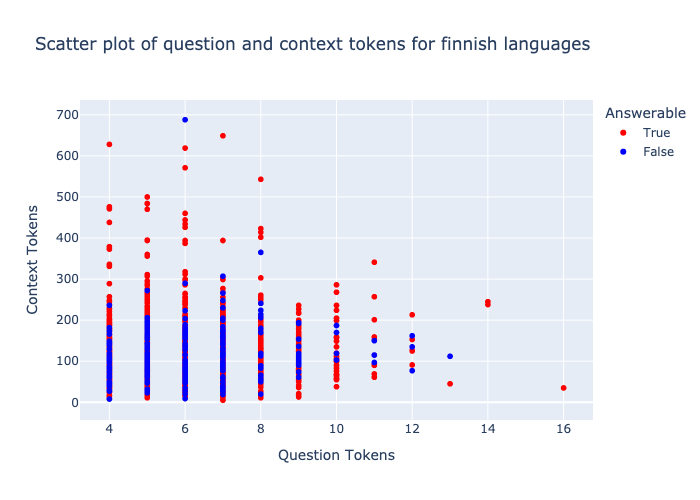
\includegraphics[width=0.5\textwidth]{week1_c_scatter_fi.png}
    \caption{Scatter plot for Finnish}
    \label{fig:scatter_week1_c_fi}
\end{figure}

\begin{figure}[ht]
    \centering
    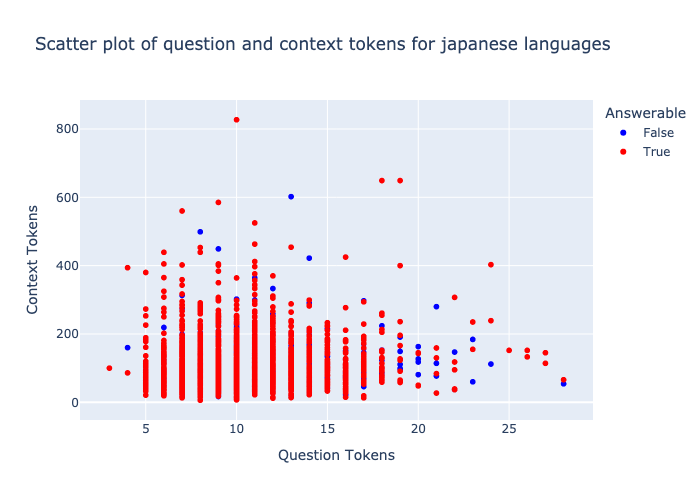
\includegraphics[width=0.5\textwidth]{week1_c_scatter_ja.png}
    \caption{Scatter plot for Japanese}
    \label{fig:scatter_week1_c_ja}
\end{figure}

\begin{figure}[ht]
    \centering
    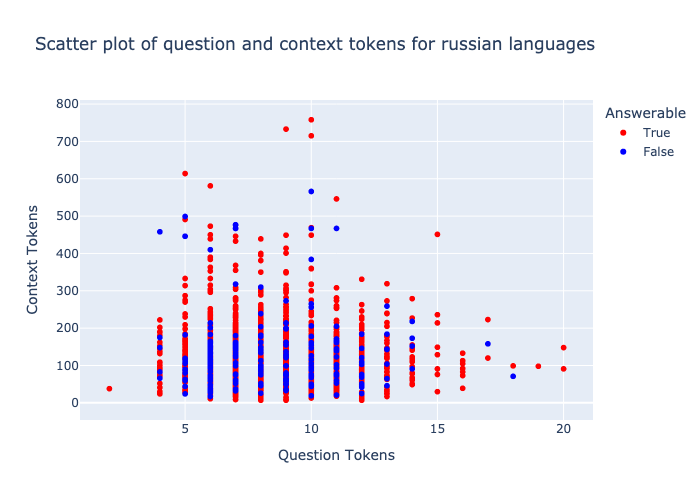
\includegraphics[width=0.5\textwidth]{week1_c_scatter_ru.png}
    \caption{Scatter plot for Russian}
    \label{fig:scatter_week1_c_ru}
\end{figure}

\begin{figure}[ht]
    \centering
    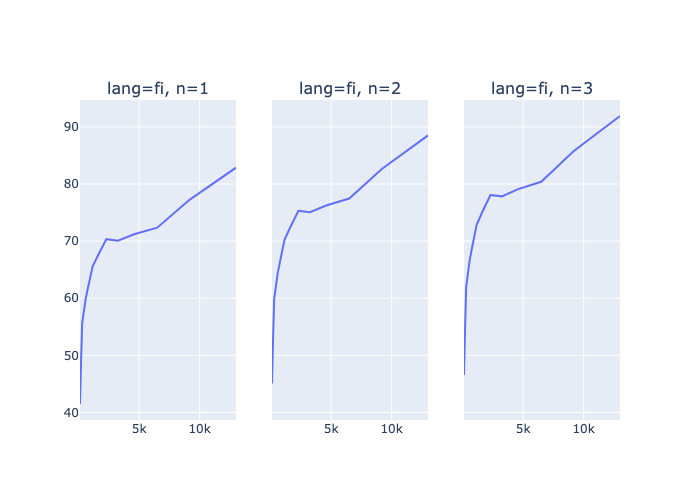
\includegraphics[width=0.5\textwidth]{week2_scaling_fi.png}
    \caption{Scaling plot for Finnish}
    \label{fig:week2_scaling_fi}
\end{figure}

\begin{figure}[ht]
    \centering
    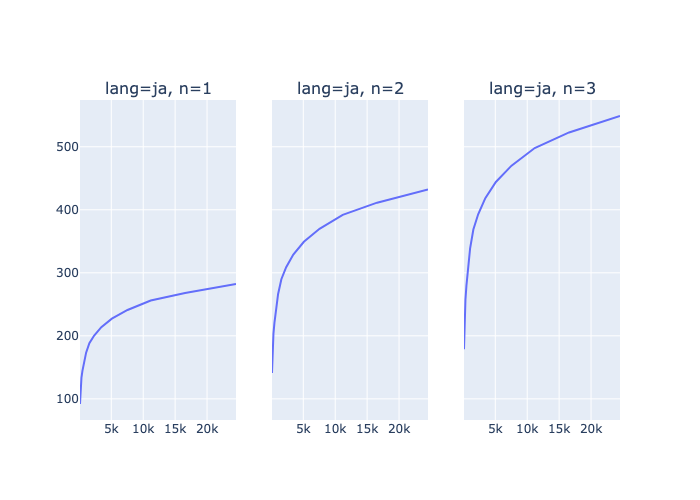
\includegraphics[width=0.5\textwidth]{week2_scaling_ja.png}
    \caption{Scaling plot for Japanese}
    \label{fig:week2_scaling_ja}
\end{figure}


\begin{figure}[ht]
    \centering
    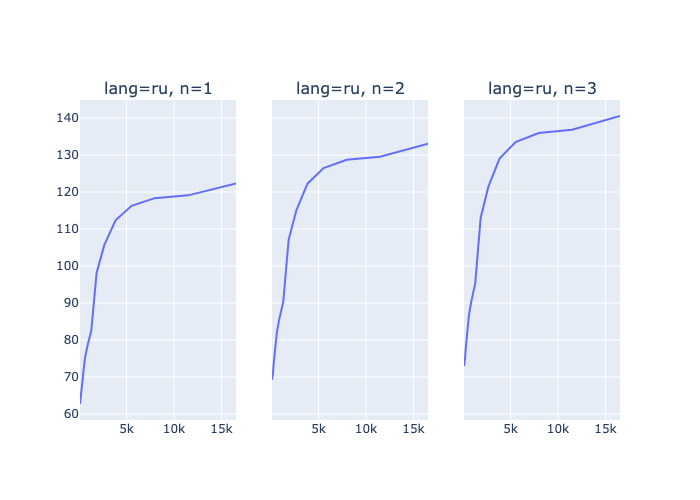
\includegraphics[width=0.5\textwidth]{week2_scaling_ru.png}
    \caption{Scaling plot for Russian}
    \label{fig:week2_scaling_ru}
\end{figure}

\begin{figure}[ht]
    \centering
    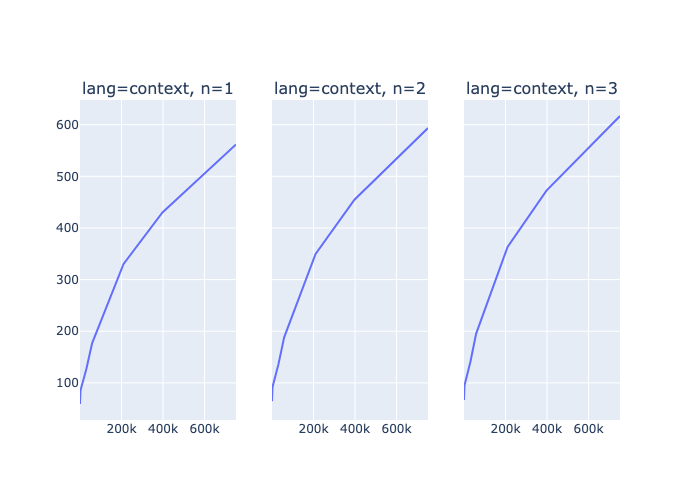
\includegraphics[width=0.5\textwidth]{week2_scaling_context.png}
    \caption{Scaling plot for context}
    \label{fig:week2_scaling_context}
\end{figure}


%% distillbert training logs

\begin{table}[ht]
    \centering
    \resizebox{0.9\columnwidth}{!}{
    \begin{tabular}{|c|c|c|c|}
        \hline
        Epoch & Language & Exact Match & F1 Score \\
        \hline
        0 & Fi & 16.10 & 17.27 \\
        0 & Ja & 19.96 & 16.49 \\
        0 & Ru & 12.88 & 17.24 \\
        \hline
        2 & Fi & 21.97 & 22.98 \\
        2 & Ja & 26.32 & 17.64 \\
        2 & Ru & 19.95 & 22.00 \\
        \hline
        4 & Fi & 27.27 & 27.39 \\
        4 & Ja & 21.27 & 19.28 \\
        4 & Ru & 18.94 & 21.50 \\
        \hline
        6 & Fi & 28.22 & 27.37 \\
        6 & Ja & 22.59 & 17.74 \\
        6 & Ru & 18.94 & 21.27 \\
        \hline
        8 & Fi & 27.27 & 26.68 \\
        8 & Ja & 23.25 & 18.49 \\
        8 & Ru & 18.43 & 22.26 \\
        \hline
        10 & Fi & 27.08 & 27.51 \\
        10 & Ja & 21.93 & 19.07 \\
        10 & Ru & 16.92 & 21.07 \\
        \hline
    \end{tabular}
    }
    \caption{Evaluation metrics for different languages at various epochs}
    \label{tab:evaluation_metrics}
\end{table}


\begin{figure}[ht]
    \centering
    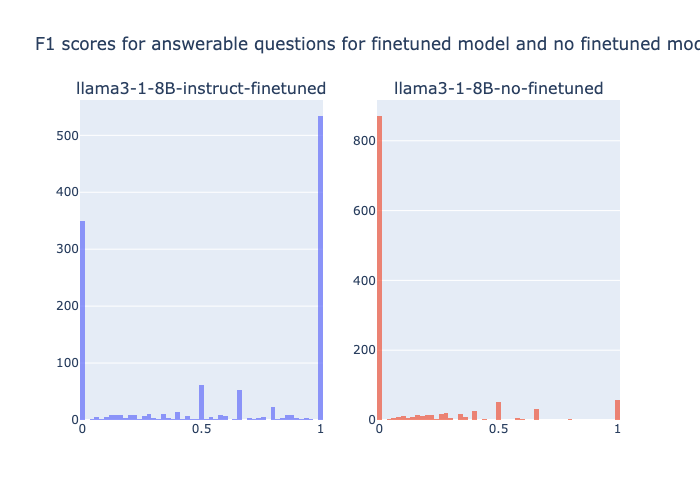
\includegraphics[width=0.5\textwidth]{week_41_f1_scores_answerable.png}
    \caption{F1 scores for answerable questions}
    \label{fig:week41_f1_scores_answerable}
\end{figure}



\subsection{References}


\subsection{Hyperlinks}
The following links provide additional resources and information related to this project:

\begin{itemize}
    \item \href{https://huggingface.co/hanspeterlyngsoeraaschoujensen}{Project Models on Hugging Face}\label{project_models_huggingface}
    \item \href{https://huggingface.co/google/mt5-base}{mT5-base model on Hugging Face}\label{mt5_base_model_huggingface}
\end{itemize}

\nocite{Ando2005,andrew2007scalable,rasooli-tetrault-2015, rajpurkar-etal-2018-know, hu2021loralowrankadaptationlarge, risch2021semanticanswersimilarityevaluating}
\section{Bib\TeX{} Files}
\label{sec:bibtex}
\bibliography{custom}
\end{document}